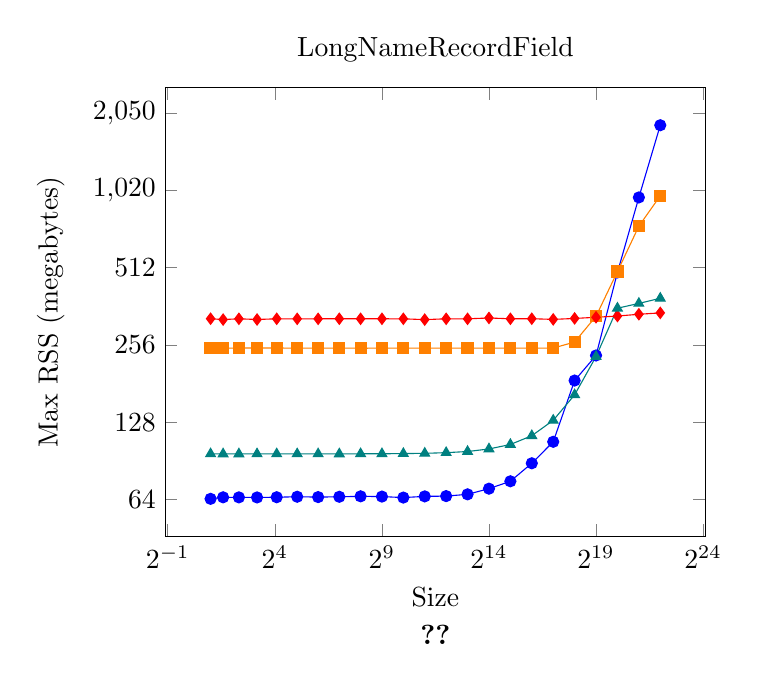
\begin{tikzpicture}
\begin{axis}
[title=LongNameRecordField,
xlabel={Size},
ylabel={Max RSS (megabytes)},
legend to name=legend,
legend columns=2,
xmode=log,
log basis x={2},
ymode=log,
log basis y={2},
yticklabel={
  \pgfkeys{/pgf/fpu=true}
  \pgfmathparse{pow(2,\tick)}
  \pgfmathprintnumber[fixed relative,precision=3]{\pgfmathresult}
  \pgfkeys{/pgf/fpu=false}
}]
\addplot [
color=blue,
mark=o,
only marks,
forget plot
] coordinates {

};
\addplot [
color=orange,
mark=square,
only marks,
forget plot
] coordinates {

};
\addplot [
color=red,
mark=diamond,
only marks,
forget plot
] coordinates {

};
\addplot [
color=teal,
mark=triangle,
only marks,
forget plot
] coordinates {

};
\addplot [
color=blue,
mark=*
] coordinates {
(4194305.0,1832.812544) 
(2097153.0,959.643648) 
(1048577.0,490.225664) 
(524289.0,232.923136) 
(262145.0,186.109952) 
(131073.0,107.47904) 
(65537.0,88.670208) 
(32769.0,75.464704) 
(16385.0,70.627328) 
(8193.0,67.137536) 
(4097.0,66.080768) 
(2049.0,65.908736) 
(1025.0,65.212416) 
(513.0,65.794048) 
(257.0,65.949696) 
(129.0,65.675264) 
(65.0,65.499136) 
(33.0,65.695744) 
(17.0,65.41312) 
(9.0,65.29024) 
(5.0,65.327104) 
(3.0,65.368064) 
(2.0,64.479232) 
};
\addlegendentry{Agda}
\addplot [
color=orange,
mark=square*
] coordinates {
(4194305.0,973.746176) 
(2097153.0,742.13376) 
(1048577.0,494.030848) 
(524289.0,330.97728) 
(262145.0,262.7584) 
(131073.0,248.832) 
(65537.0,248.643584) 
(32769.0,248.89344) 
(16385.0,248.877056) 
(8193.0,248.807424) 
(4097.0,248.815616) 
(2049.0,248.922112) 
(1025.0,248.655872) 
(513.0,248.700928) 
(257.0,248.553472) 
(129.0,248.91392) 
(65.0,248.85248) 
(33.0,248.85248) 
(17.0,248.967168) 
(9.0,248.967168) 
(5.0,248.958976) 
(3.0,248.766464) 
(2.0,248.655872) 
};
\addlegendentry{Idris 2}
\addplot [
color=red,
mark=diamond*
] coordinates {
(4194305.0,341.123072) 
(2097153.0,336.912384) 
(1048577.0,331.603968) 
(524289.0,328.011776) 
(262145.0,324.550656) 
(131073.0,321.80224) 
(65537.0,323.784704) 
(32769.0,323.567616) 
(16385.0,325.87776) 
(8193.0,323.493888) 
(4097.0,323.497984) 
(2049.0,321.138688) 
(1025.0,323.465216) 
(513.0,323.54304) 
(257.0,323.493888) 
(129.0,323.6864) 
(65.0,323.493888) 
(33.0,323.489792) 
(17.0,323.510272) 
(9.0,321.536) 
(5.0,323.526656) 
(3.0,321.314816) 
(2.0,323.756032) 
};
\addlegendentry{Lean 4}
\addplot [
color=teal,
mark=triangle*
] coordinates {
(4194305.0,388.825088) 
(2097153.0,371.388416) 
(1048577.0,355.71712) 
(524289.0,230.760448) 
(262145.0,163.708928) 
(131073.0,130.256896) 
(65537.0,113.496064) 
(32769.0,104.927232) 
(16385.0,100.794368) 
(8193.0,98.5088) 
(4097.0,97.509376) 
(2049.0,96.93184) 
(1025.0,96.722944) 
(513.0,96.538624) 
(257.0,96.538624) 
(129.0,96.407552) 
(65.0,96.436224) 
(33.0,96.436224) 
(17.0,96.432128) 
(9.0,96.432128) 
(5.0,96.403456) 
(3.0,96.407552) 
(2.0,96.468992) 
};
\addlegendentry{Rocq}
\end{axis}
\node[anchor=north] at (current axis.below south) {\ref{legend}};
\end{tikzpicture}
